%------------------------
% CV in Latex
% Author: Sourabh Bajaj
% Modified by: Abhishek Ramanathapura Satyanarayana
% License: MIT
%------------------------

\documentclass[letterpaper, 11pt]{article}

\usepackage{latexsym}
\usepackage[empty]{fullpage}
\usepackage{titlesec}
\usepackage{marvosym}
% \usepackage[usenames,dvipsnames]{color}
\usepackage{xcolor}
\usepackage{verbatim}
\usepackage{enumitem}
\usepackage[pdftex]{hyperref}
\usepackage{fancyhdr}
\usepackage{ragged2e}
\usepackage{comment}
\usepackage{graphicx,wrapfig}
\usepackage{fontawesome}
\graphicspath{{./images/}}

\pagestyle{plain}
\fancyhf{} % clear all header and footer fields
\fancyfoot{}
\cfoot{\thepage}
\renewcommand{\headrulewidth}{0pt}
\renewcommand{\footrulewidth}{0pt}

% Adjust margins
% \addtolength{\oddsidemargin}{-0.375in}
% \addtolength{\evensidemargin}{-0.375in}
% \addtolength{\textwidth}{1in}
% \addtolength{\topmargin}{-.5in}
% \addtolength{\textheight}{1.0in}
\usepackage[margin=0.6in]{geometry}

\urlstyle{same}
\raggedbottom
\raggedright
\setlength{\tabcolsep}{0in}

% Sections formatting
\titleformat{\section}{
    \vspace{-4pt}\scshape\filcenter\large
}{}{0em}{}[\color{black}\titlerule \vspace{-5pt}]

%-------------------------
% Custom commands
\newcommand{\resumeItem}[2]{
    \item\small{
        \textbf{#1}{: #2 \vspace{-2pt}}
    }
}

\newcommand{\resumeSubheading}[4]{
    \vspace{-1pt}\item
    \begin{tabular*}{0.97\textwidth}{l@{\extracolsep{\fill}}r}
        \textbf{#1} & #2 \\
        \textit{\small#3} & \textit{\small #4} \\
    \end{tabular*}\vspace{-5pt}
}

\newcommand{\resumeSubItem}[2]{\resumeItem{#1}{#2}\vspace{-4pt}}

\renewcommand{\labelitemii}{$\circ$}

\newcommand{\resumeSubHeadingListStart}{\begin{itemize}[leftmargin=*]}
\newcommand{\resumeSubHeadingListEnd}{\end{itemize}\vspace{-5pt}}
\newcommand{\resumeItemListStart}{\begin{itemize}}
\newcommand{\resumeItemListEnd}{\end{itemize}\vspace{-5pt}}
\definecolor{navy_blue}{HTML}{006EB8}

%-------------------------------------------
%%%%%%  CV STARTS HERE  %%%%%%%%%%%%%%%%%%%%%%%%%%%%
\pagenumbering{gobble}

\begin{document}



%--------IMAGE_AT_TOP_RIGHT--------
\begin{comment}
    \begin{wrapfigure}[1]{r}{0.10\textwidth}
        \centering
        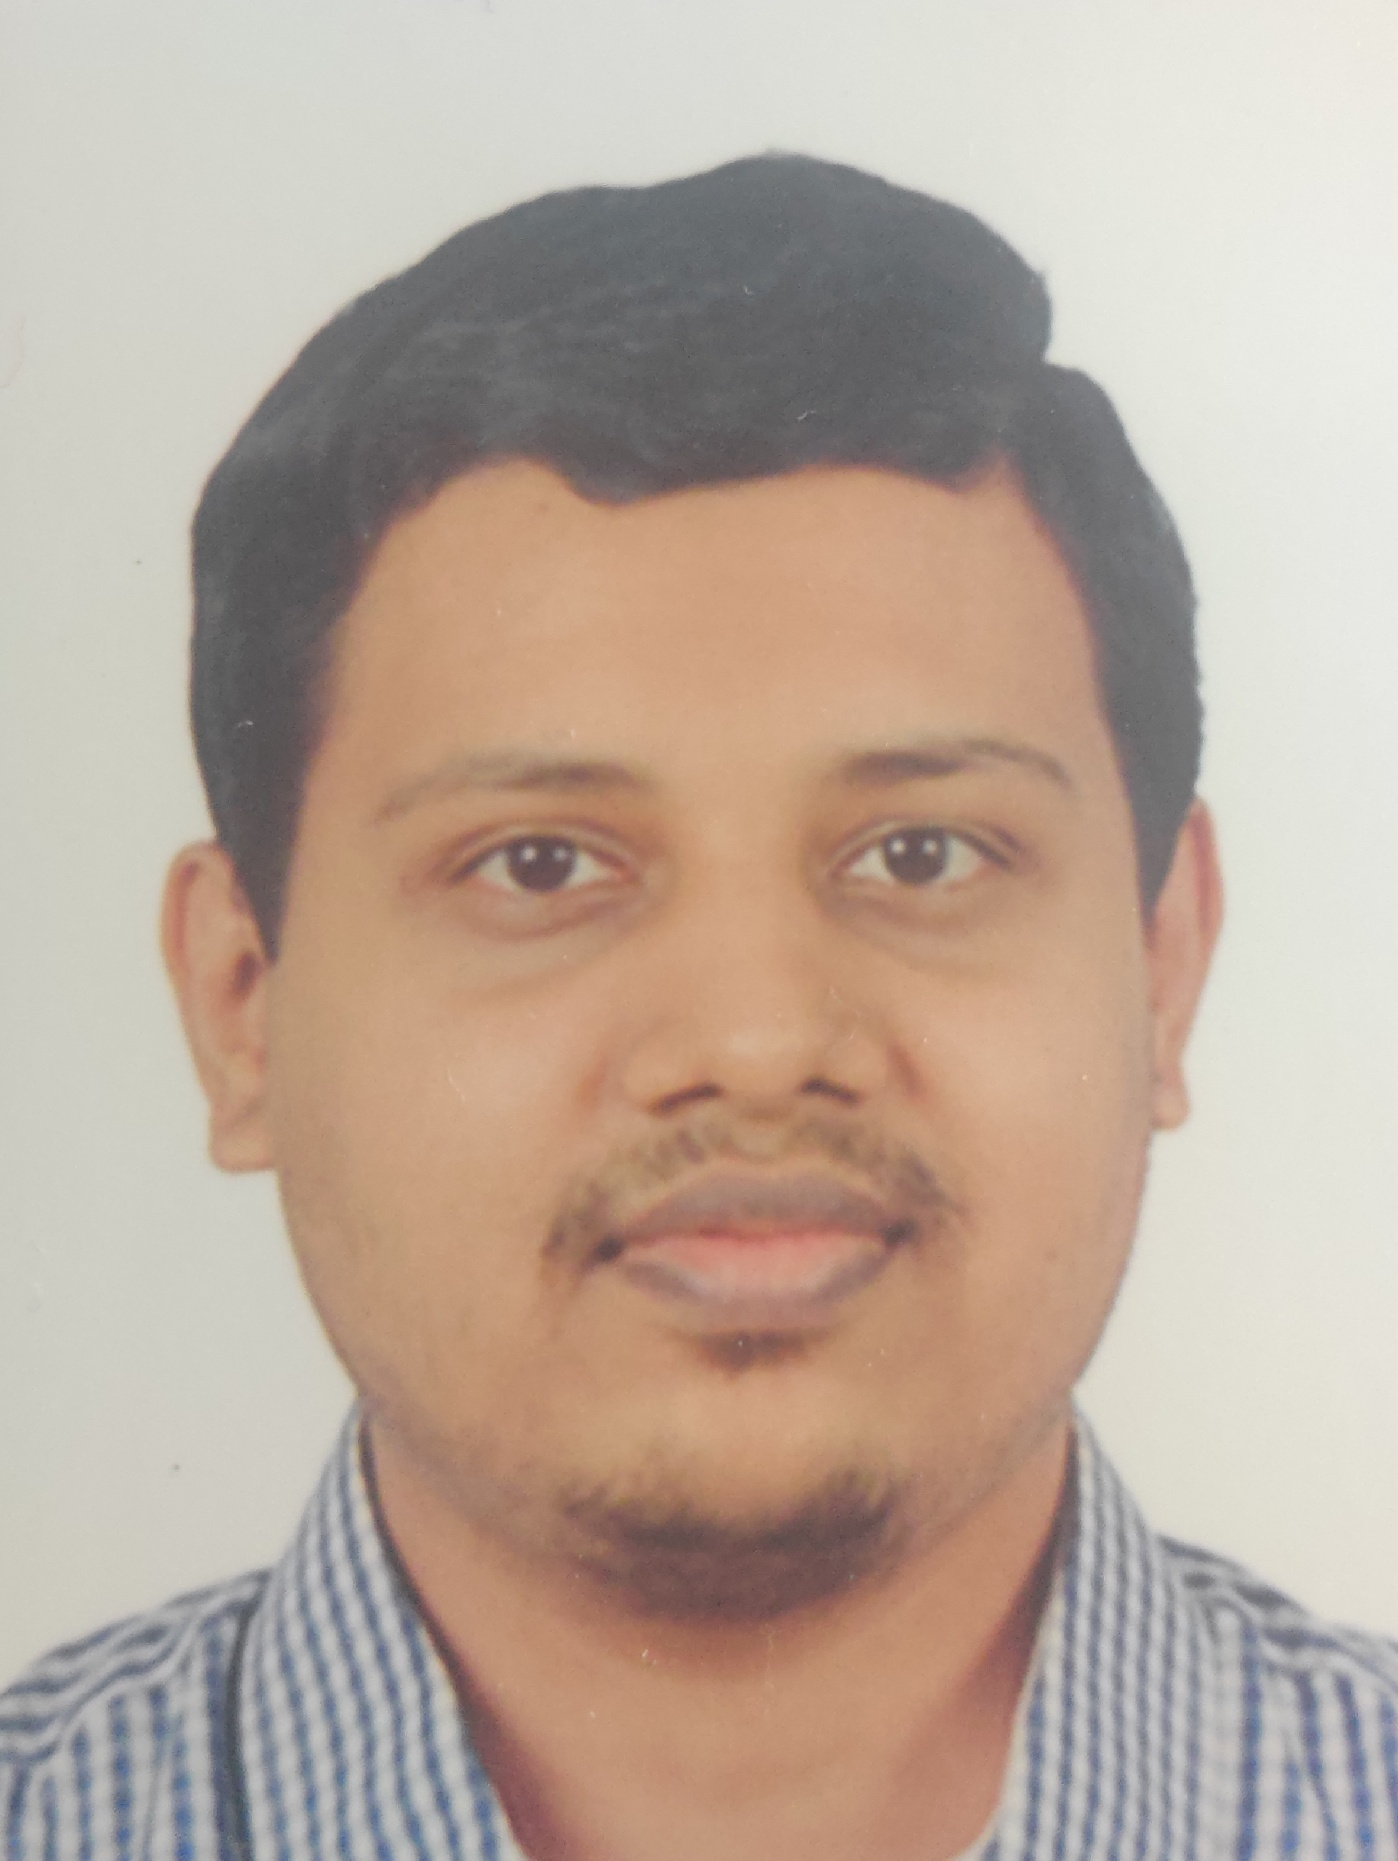
\includegraphics[width=1\linewidth]{images/abhishek_r_s.jpg}
    \end{wrapfigure}
    \paragraph{}
\end{comment}



%----------HEADING-----------------
\begin{tabular*}{\textwidth}{l@{\extracolsep{\fill}}r}
    \textcolor{navy_blue}{\textbf{{\Large Abhishek Ramanathapura Satyanarayana}}}
    \\
    {(+91) 9036431474, Bengaluru, India (willing to relocate)}
    \vspace{0.15cm}
    \\
    
    \textbf{Email}: \href{mailto:abhishek.r.satyanarayana.4@gmail.com}{abhishek.r.satyanarayana.4@gmail.com} \hspace{0.1cm} 
    % \href{mailto:abhishekrsatyanarayana@gmail.com}{\faEnvelope} \hspace{0.1cm}
    \\
    \textbf{GitHub}: \href{https://github.com/AbhishekRS4/}{https://github.com/AbhishekRS4/} \hspace{0.1cm} 
    \textbf{HuggingFace}: \href{https://huggingface.co/abhishekrs4}{https://huggingface.co/abhishekrs4}
    \\
    \textbf{Personal Website}: \href{https://abhishekrs4.github.io/}{https://abhishekrs4.github.io/} \hspace{0.1cm} 
    \textbf{LinkedIn}: \href{https://linkedin.com/in/abhishek-r-s/}{https://linkedin.com/in/abhishek-r-s/} \hspace{0.1cm}
    %\href{https://drive.google.com/drive/folders/0Byk-dMy2pBxeX21IbmRlWFExNFk?usp=sharing}{\faFilesO}
    \\
\end{tabular*}



%----------PROFESSIONAL SUMMARY-----------------
\section{\textbf{\textcolor{navy_blue}{* PROFESSIONAL SUMMARY *}}}

\justifying{I am a growing AI Engineer with an interest in the intersection of AI, Machine Learning, Deep Learning, Computer Vision, and Data Science domains. I have constantly demonstrated my skills by adding value to the company and other stakeholders by developing and deploying AI, Machine Learning, Deep Learning, and Computer Vision solutions at work and internship. As a data specialist, I am interested in the long-term goal of improving human lives through continuous development and deployment of data-driven applications that have a significant impact on the real world and drive business growth by adding value to all stakeholders.}



%----------SKILLS-----------------
\section{\textbf{\textcolor{navy_blue}{* SKILLS *}}}

    \resumeSubHeadingListStart
        \resumeSubItem{Programming languages}{Python, C++, C}
        \resumeSubItem{Version control (CI/CD)}{Git, GitHub}
        \resumeSubItem{ML / MLOps Tools}{PyTorch, TensorFlow, Transformers, Scikit-learn, MLFlow, Weights and Biases}
        \resumeSubItem{Web Frameworks}{Streamlit, Flask, FastAPI}
        \resumeSubItem{Data Manipulation and Visualization}{Numpy, Scipy, Pandas, Matplotlib, Seaborn, OpenCV}
        \resumeSubItem{Miscellaneous tech}{Linux, TensorRT, Docker, HuggingFace, AWS, Prefect, PyLint, PyTest}
        \resumeSubItem{Soft skills}{Teamwork, Time management, Communication, Leadership, Business acumen}
        \resumeSubItem{Languages}
        {English (professional), Dutch (elementary), Kannada (native), Hindi (professional)}
    \resumeSubHeadingListEnd



%-----------PROFESSIONAL EXPERIENCE-----------------
\section{\textbf{\textcolor{navy_blue}{* PROFESSIONAL EXPERIENCE *}}}
    \resumeSubHeadingListStart
        \resumeSubheading{Data Scientist - 2}{Bengaluru, India}{SatSure}{Mar 2025 - Present}
            \resumeSubHeadingListStart
                \resumeItem{Responsibilities}{I am currently working in the R \& D Data Science development team at SatSure. I am working to leverage satellite data, geospatial data, and data from other sources to develop and deploy next-generation data-driven products and solutions for diverse use cases for earth observation.}
            \resumeSubHeadingListEnd
    
        \resumeSubheading{Teaching Assistant (Part-time)}{Groningen, The Netherlands}{Faculty of Science and Engineering [FSE], University of Groningen}{Sep 2022 - Jun 2023}
            \resumeSubHeadingListStart
                \resumeItem{Responsibilities}{I monitored the weekly lab sessions, mentored some students and teams in their course projects, and graded the course projects and assignments. I worked as a TA for the following courses.}
                \resumeItem{Courses}{Cognitive Robotics, Introduction to Data Science, Deep Learning, Computer Vision, Handwriting Recognition.}
            \resumeSubHeadingListEnd
    
        \resumeSubheading{Summer AI Intern}{IJmuiden, The Netherlands}{Tata Steel in Europe}{Jul 2022 - Aug 2022}
            \resumeSubHeadingListStart
                \resumeItem{Responsibilities}{This summer internship was a part of the \href{https://www.summerof.ai/}{Dutch Summer of AI}, edition 2022. I worked on supervised and unsupervised deep learning methods to classify and cluster images with steel surface defects. For the unsupervised task, I worked on a proof-of-concept model. For the supervised steel surface defect classification task, I worked on developing a production-ready AI model that achieved a $92\%$ accuracy, higher than that of the baseline model. \textbf{When deployed, this model would save at least $\mathbf{500}$K Euros annually for Tata Steel}. Our team won the award for \textbf{Solving the Most Valuable Problem}.}
                \resumeItem{Skills}{Teamwork, Time management, Communication, Presentation, Python, PyTorch, MLFlow.}
            \resumeSubHeadingListEnd

        \resumeSubheading{Teaching Assistant (Part-time)}{Groningen, The Netherlands}{University Medical Center Groningen [UMCG], University of Groningen}{Jun 2022 - Jul 2022}
            \resumeSubHeadingListStart
                \resumeItem{Responsibilities}{I worked as a TA for the Summer School of Data Science and AI in Health. I was responsible for setting up the assignment notebooks. I monitored and helped the students during the summer school.}
            \resumeSubHeadingListEnd

        \resumeSubheading{Project Intern}{Drachten, The Netherlands}{Philips}{Nov 2021 - Jul 2022}
            \resumeSubHeadingListStart
                \resumeItem{Responsibilities}{This internship was part of the HTSM programme at the University of Groningen. I worked on a project report proposing ways to develop a more sustainable shaver with less carbon footprint. \textbf{The top 3 solutions that our team proposed could reduce the carbon footprint of the shaver by at least 10-20\% depending on the solution}.}
            \resumeSubHeadingListEnd

        \resumeSubheading{Machine Learning Research Associate}{Bengaluru, India}{Ati Motors}{Sep 2017 - Jun 2021}
            \resumeSubHeadingListStart
                \resumeItem{Responsibilities}
                {Ati Motors is a startup working on the development and deployment of autonomous cargo electric vehicles to automate material movement in warehouse, factory, and industrial settings. I worked mainly on research, prototyping, development, and deployment of machine learning, deep learning, computer vision, robot perception, and various algorithms solutions for autonomous cargo vehicles in the Autonomy team.}
                \resumeItem{Notable Contributions}
                {My contributions include developing and deploying obstacle classification, obstacle detection, road segmentation, and lane segmentation models using 2D camera images, and a drivable area segmentation model using 3D LiDAR point cloud data. I benchmarked various ML models on different hardware devices such as multiple Nvidia GPUs, Intel Movidius stick, and Nvidia Xavier embedded development board. I also contributed to the development, deployment, and testing of the raw and derived sensor data pipelines of the LiDAR and camera sensors. \textbf{Much of my contributions translated into Ati showcasing more than 15 demos at potential customer sites and Ati’s first 3 successful customer deployments. The total number of customer deployments has increased now.}}
                \resumeItem{Skills}{Communication, Teamwork, Linux, Docker, GitHub, C++, C, Python, PyTorch, TensorFlow, MLFlow, OpenCV, TensorRT, Streamlit, Flask, AWS.}
            \resumeSubHeadingListEnd

    \resumeSubHeadingListEnd



%-----------PROJECTS-----------------
\begin{comment}
\section{\textbf{\textcolor{navy_blue}{* PROJECTS *}}}
    \resumeSubHeadingListStart
        \resumeSubItem{Oil Spill Segmentation}{Developed and deployed an AI based computer vision application using deep learning to detect and segment the oil spills in the images extracted from Synthetic Aperture Radar (SAR) data. The streamlit application is deployed to HuggingFace.}
        \resumeSubItem{Handwriting Recognition}{Developed and deployed an AI based computer vision application using deep learning to recognize handwritten English language text in the images trained using the IAM dataset. The Flask and streamlit applications are deployed to HuggingFace.}
        \resumeSubItem{Image Colourization with CGAN}{Developed and deployed an AI based computer vision application using deep learning to generate colourized images for the grayscale images. The CGAN was trained using the COCO dataset. The FastAPI application is deployed to HuggingFace.}
    \resumeSubHeadingListEnd
\end{comment}


%------------EDUCATION-----------------
\section{\textbf{\textcolor{navy_blue}{* EDUCATION *}}}
    \resumeSubHeadingListStart
        \resumeSubheading
            {M.Sc. in Artificial Intelligence}{Groningen, The Netherlands}
            %{\underline{\href{https://www.rug.nl/masters/artificial-intelligence/}{University of Groningen [RUG]}}}{Sep 2021 - present}
            {University of Groningen [RUG]}{Sep 2021 - Oct 2023}
            \resumeSubHeadingListStart
                \resumeItem{Thesis}{For my AI Master's thesis I worked on a research project titled \textbf{Enhancing Depth Estimation for Transparent Objects}. In this research, I proposed a novel encoder-decoder architecture that outperformed the state-of-the-art method.}
                \resumeItem{Grade}{GPA: 8.3/10, Thesis: 8.5/10, \textbf{graduated cum laude}}
                \resumeItem{Awards}{\textbf{One of the best student project awards in NLP course} and \textbf{second best performer student project award in the Intro to Data Science course.}}
            \resumeSubHeadingListEnd

        \resumeSubheading
            {Honours Master's in High Tech Systems and Materials (HTSM)}{Groningen, The Netherlands}
            %{\underline{\href{https://www.rug.nl/education/honours-college/htsm-masterprogramme/}{Honours College, University of Groningen}}}{Nov 2021 - Jun 2023}
            {Honours College, University of Groningen}{Nov 2021 - Jun 2023}
            \resumeSubHeadingListStart
                \resumeItem{Masterwork}{For my HTSM Masterwork, I worked on a project titled \textbf{Oil Spill Segmentation using Deep Encoder-Decoder models}. In this project, I developed and evaluated the performance of popular deep encoder-decoder models for the oil spill segmentation task. The best-performing model has been deployed to HuggingFace.}
                \resumeItem{Grade}{GPA: 7.9/10, Masterwork: 9/10}
            \resumeSubHeadingListEnd
        
        \resumeSubheading
            {B.Tech. in Information Technology}{Surathkal, Mangaluru,  India}
            %{\underline{\href{https://www.nitk.ac.in/}{National Institute of Technology Karnataka [NITK]}}}{Jul 2012 - May 2016}
            {National Institute of Technology Karnataka [NITK]}{Jul 2012 - May 2016}
            \resumeSubHeadingListStart
                \resumeItem{Grade}{CGPA: 8.3/10}
            \resumeSubHeadingListEnd
    \resumeSubHeadingListEnd


\begin{comment}
% --------REFERENCES------------
\section{\textbf{\textcolor{navy_blue}{* REFERENCES *}}}
    \resumeSubHeadingListStart
        \item
        {Dr. Hamidreza Kasaei \\
        Assistant Professor \\
        Faculty of Science and Engineering \\
        University of Groningen, Groningen, The Netherlands \\
        Email: \underline{\href{mailto:hamidreza.kasaei@rug.nl}{hamidreza.kasaei@rug.nl}} \\
        Website: \underline{\href{https://www.rug.nl/staff/hamidreza.kasaei/}{https://www.rug.nl/staff/hamidreza.kasaei/}}}
        \item
        {Dr. Maruf Dhali \\
        Assistant Professor \\
        Faculty of Science and Engineering \\
        University of Groningen, Groningen, The Netherlands \\
        Email: \underline{\href{mailto:m.a.dhali@rug.nl}{m.a.dhali@rug.nl}} \\
        Website: \underline{\href{https://www.rug.nl/staff/m.a.dhali/}{https://www.rug.nl/staff/m.a.dhali/}}}
    \resumeSubHeadingListEnd    
\end{comment}



\end{document}
